\chapter{Normalized Measurements}\label{chap:normalized}
This chapter explains the procedure for normalized measurements. The first section gives a layout for both hardware and software implementation of the normalized measurements and is followed by a short explanation to \acs{EIRP} measurement. Then the next section defines the link-budget for this approach. The fourth section demonstrates the normalization procedure. Following this explains the optimization of the antenna pair. The final section illustrates the program for the selection of the best-required probe antennas.


\section{Implementation}
The flow chart in Figure \ref{fig:1} explains the procedure for normalized measurements. Each step in the flowchart is further explained in detail in the further sections of this chapter. For the normalization measurements, the first step is to find the \acs{EIRP} of the \acs{DUT}. This can be done by a conducted measurement or by simply measuring the \acs{EIRP} in an \acf{AC}. The later provides us with the radiation pattern of the \acs{DUT}.  The \acs{EIRP} measurement is just done once for each \acs{DUT} and the results are normalized using this \acs{EIRP} value of the \acs{DUT}. Before performing the normalized measurements, it is important to find the best configuration for the cables and connections. This step is also done only once and all other measurements are done using the same configuration of the instruments and cables. This step also includes the calibration of all the cables within the system.  The section \ref{sec:opti} explains the above procedure.

\begin{figure}[H]
\centering
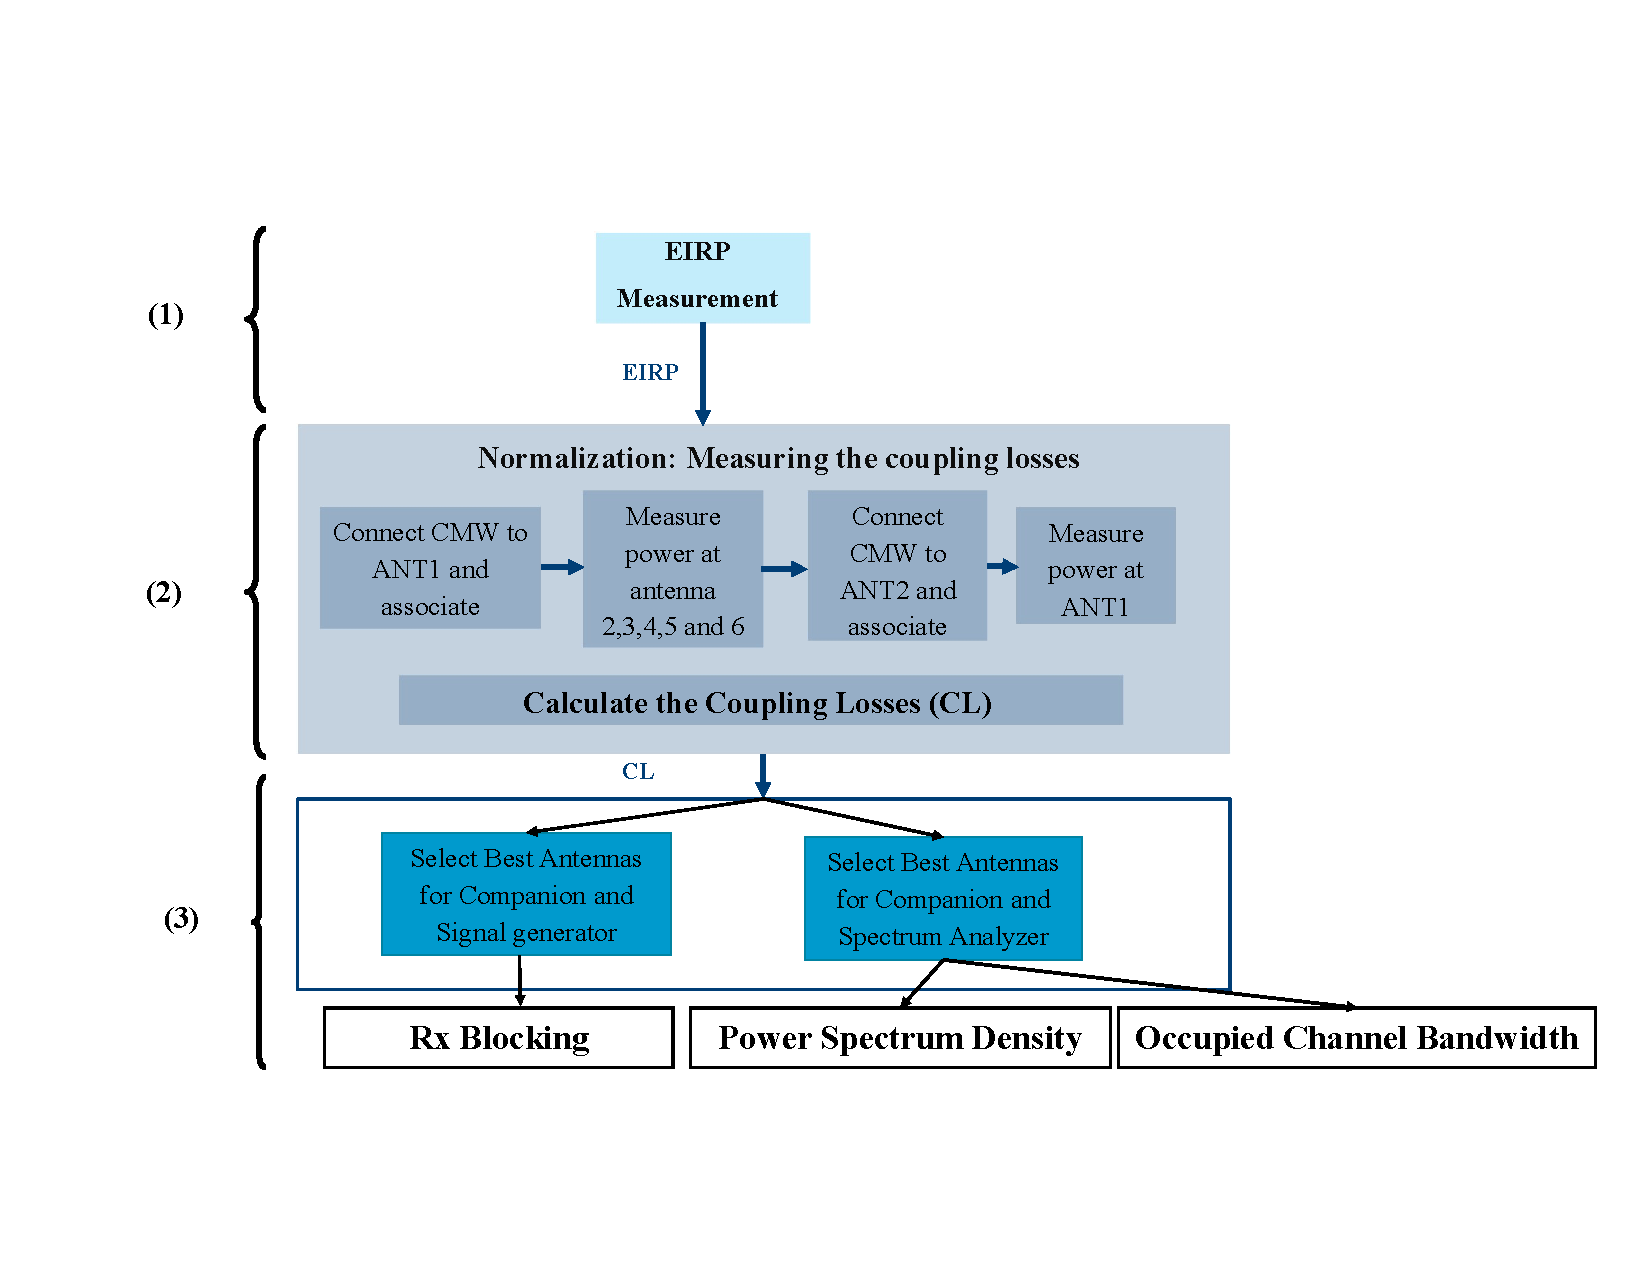
\includegraphics[scale = 0.65]{normflowchart.pdf}
\vspace{-2cm} \caption{Flowchart explaining the novel approach for wireless coexistence testing}
\label{fig:1} 
\end{figure}

The second block (2) in the flow chart \ref{fig:1} is explained in the section called Normalization. This procedure is vital for these measurements. This step is done every time a new test is run. Sometimes, long term measurements are done so that the \acf{MU} for the particular test case can be evaluated. This step then is performed at the beginning of the long term measurement and therefore the resulting coupling loss is used for all the measurement times during that long term measurement. \\
 
The selection of the best antenna probe depends mainly on the test case specification. For example, the companion device and the spectrum analyzer is used for \acf{OBW} measurement and \acf{PSD} measurement. And, the Receiver Blocking test case uses the companion device along with the signal generator. Each instrument usually is confined to 2 antenna ports due to the internal block diagram of the switching module (explained in section \ref{sec:wn}). The procedure for the selection is explained in the sub-topic called the selection of the best probe antenna. The measurement is run after all the mentioned steps. To get a good idea of the \acf{MU}, each test measurement is run several times, and the mean and standard deviation is computed. \\

This section also gives a brief overview of the implementation of the developed MATLAB\textregistered{} tool. The Figure \ref{fig:2} shows the individual steps of the measurement process implemented in this thesis.

\begin{figure}[H]
\centering
\includegraphics[scale = 0.6]{arrow.pdf}
\vspace{-2cm}\caption{Flow of the automation software}
\label{fig:2} 
\end{figure}

The software tool for automated wireless coexistence measurement is implemented in MATLAB\textregistered{} because of several reasons. MATLAB\textregistered{} is a numerical computing environment and fourth-generation programming language allowing matrix manipulations, plotting of acquired data, implementation, and testing of algorithms (e.g. for signal processing and antenna radiation patterns). One big advantage of MATLAB\textregistered{} is the availability of commonly used functions that are already implemented in the MATLAB\textregistered{} environment. Additionally, there are many toolboxes available, which are either free or can be purchased from MathWorks or third party suppliers. \acs{RS}\textregistered{} has many of these additional toolboxes licensed, which reduces development time significantly. This is especially important when studying new approaches as in the case of this thesis.

\subsection{Hardware Design}
The steps for implementation of radiated measurements are explained as follows:
\begin{enumerate}
  \item Place the \acs{DUT} inside an \acf{AC} and measure the maximum \acs{EIRP} from the \acs{DUT}.
  \item Place the \acs{DUT} in the \acs{RF} shielded box and connect the instruments as shown in the block diagram.

\begin{figure}[H]
\centering
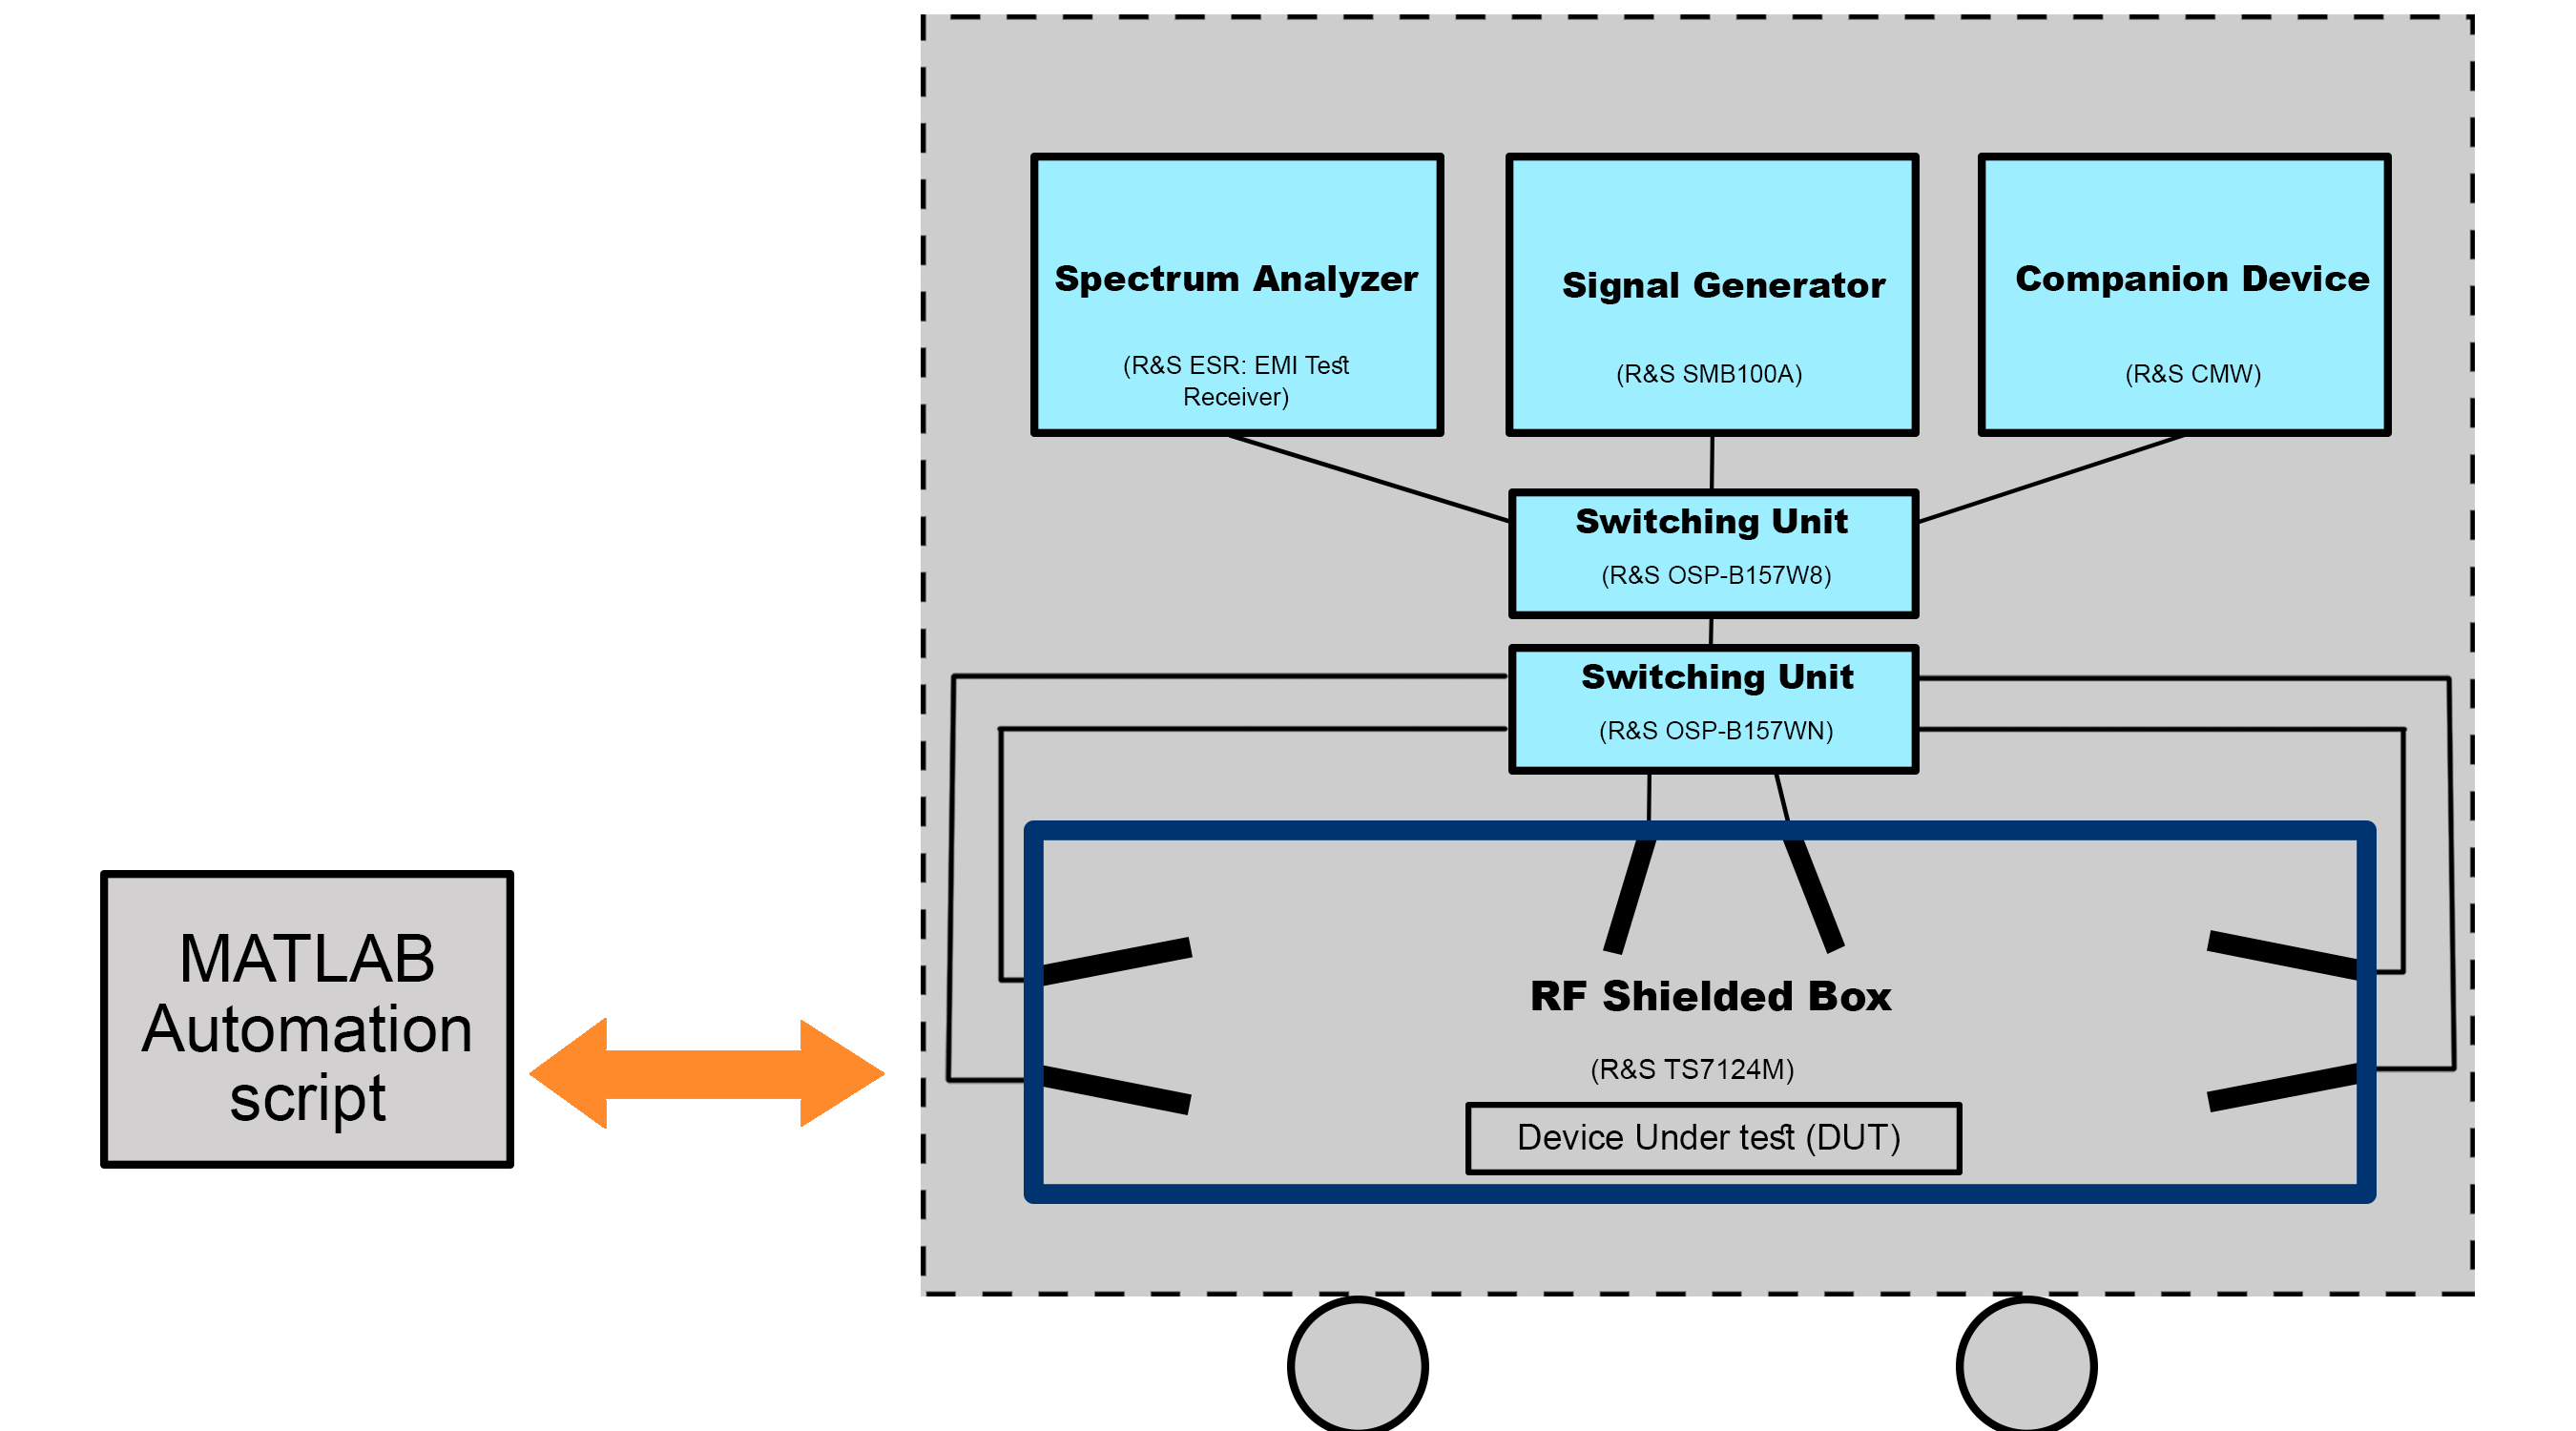
\includegraphics[scale = 0.18]{hwdesign.png}
\caption{Design for the implementation of the wireless coexistence system}
\label{fig:3} 
\end{figure}

There are six probe antennas inside the \acs{RF} shielded box. They work in pairs of 2. i.e. 2 antennas for spectrum analyzer which is used for measuring the power, bandwidth, etc. 2 other antennas are used for injecting a signal which is used in case of receiver blocking or adaptivity test case. And finally, the last pair of antennas are used for communicating with the \acs{DUT} by the companion device.

\item Perform Normalization: Power, which is found by calculating the average of each burst of the \acs{DUT} signal and finding the maximum of all bursts, is measured at all six antennas. The difference between the measured \acs{EIRP} in step 1 and the power measured at each antenna is defined as the coupling loss for that particular path. This step is explained in detail in the next section.

\item Select the best probe antenna out of each pair of antennas depending on the different test cases. The best probe antenna is considered the one which has minimum coupling loss. This step is explained in section \ref{sec:sba}. 

\item Run a measurement from the decided test cases. The procedure for each test case is explained in chapter \ref{chap:test}.

\end{enumerate}



\subsection{Software Design}
After the conducted measurement analysis was fundamentally verified in the experimental setup, the software implementation was restructured. Since the complexity of the implementation grew over time, an object-oriented programming style is used in the current implementation to account for this development. The object-oriented design improves the understanding of the code because the structure represents the real nature of the data well.

When one creates a class in MATLAB\textregistered{}, it is by default a value class. I prefer having to update objects by reference, therefore the class uses a handle class. This can made a handle class by changing the first line to:
\begin{lstlisting}[language=MATLAB]
classdef testClass < handle
\end{lstlisting}
Also, one wouldn't necessarily need output arguments for the methods of the handle class which is one of the main reasons for using this class. 

\begin{figure}[H]
\centering
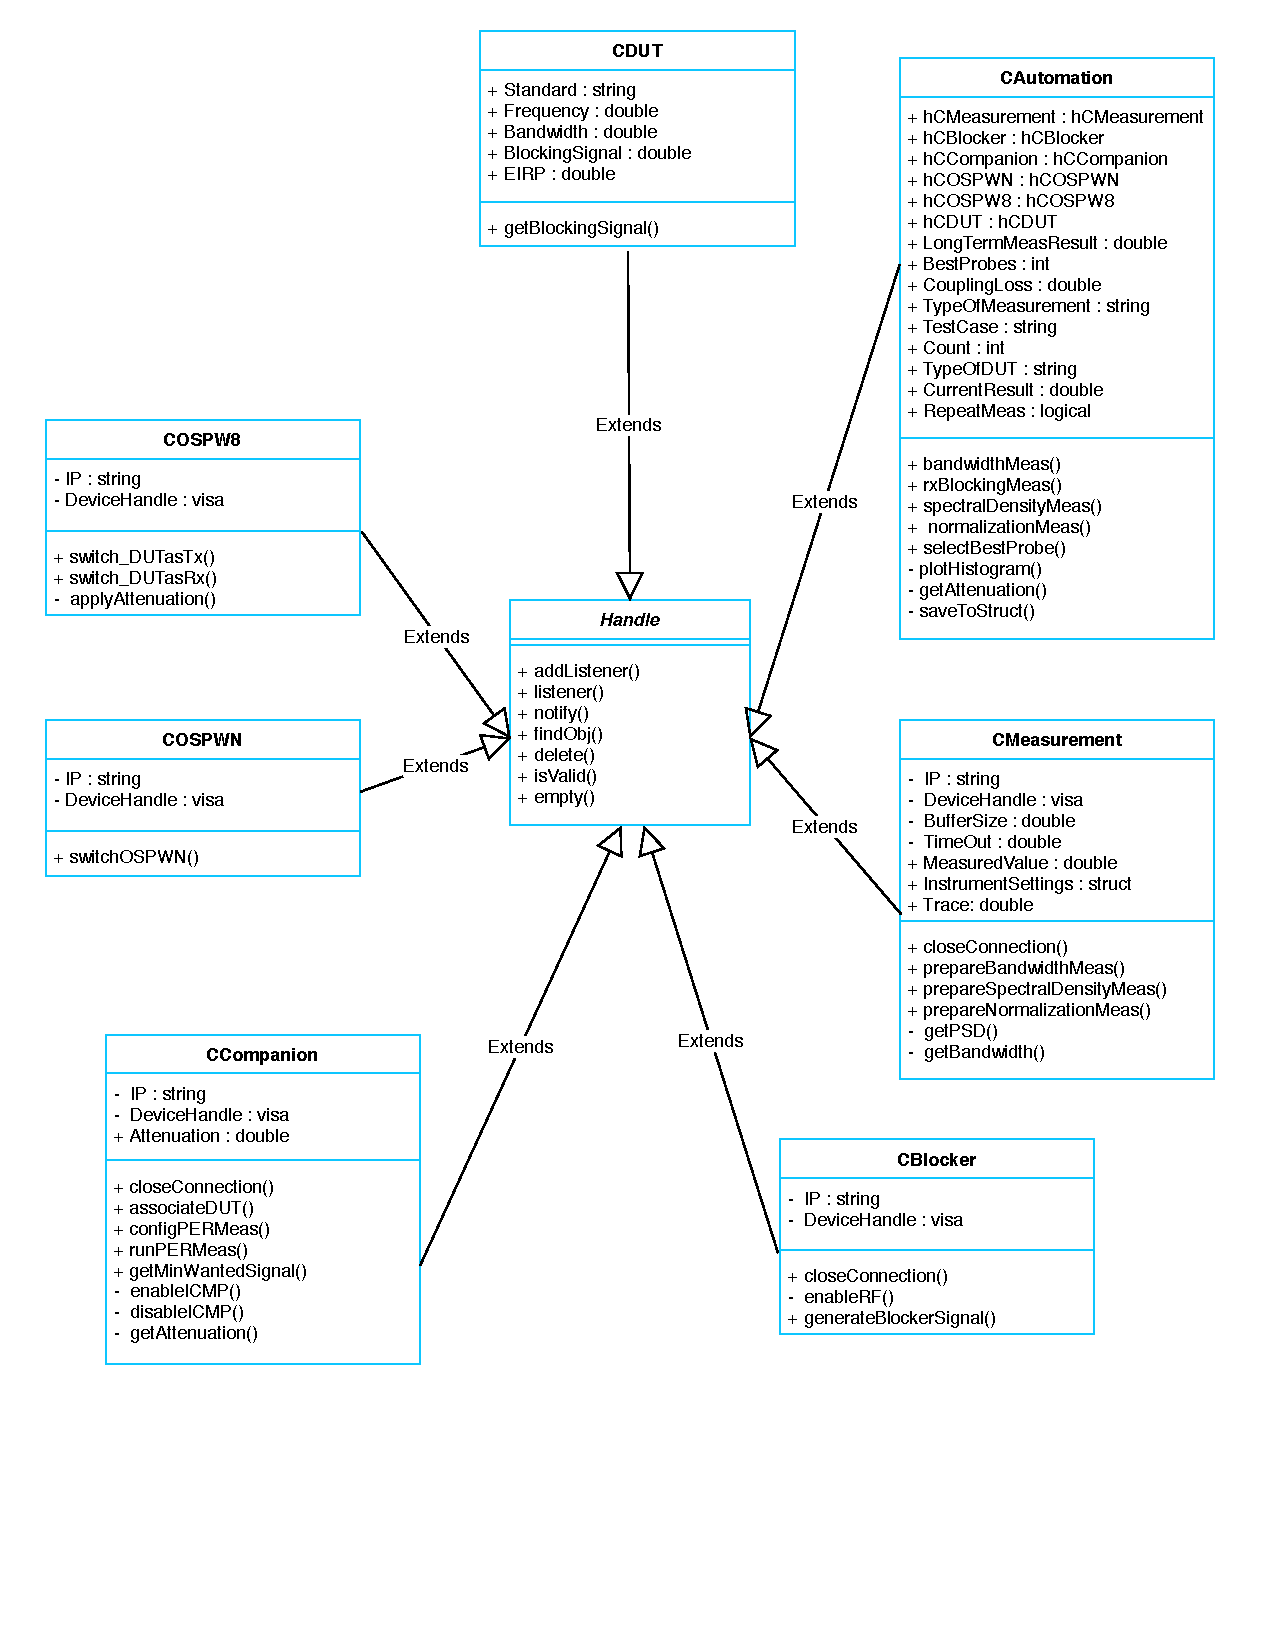
\includegraphics[scale = 0.65]{ClassDiagram.pdf}
\caption{UML Class Diagram}
\label{fig:cd} 
\end{figure}

The seven classes build the core of the developed software tool . For better overview and understanding some attributes and methods are omitted in this class diagram (Figure \ref{fig:cd}). Each of these classes is derived from the base class Handle. The CAutomation class instantiates objects from all the other six classes. Five of those classes are the instruments used in this thesis, i.e., Spectrum Analyzer, Signal Generator, Connectivity Tester, two Switching modules, and the last class named CDUT, specifies the \acs{DUT} standard, operating frequency, bandwidth, \acs{EIRP}, and so on.

\section{\acs{EIRP} Measurement}
\acs{EIRP} is measured once for every \acs{DUT} used. Maximum \acs{EIRP} is generally measured using \acs{OTA} measurements.  But, in this case the \acs{EIRP} estimation is done by measuring the conducted output power and applying the stated antenna gain. The Figure \ref{fig:Ng1} explains the implementation of this measurement. The \acs{DUT} is associated with the companion device via a \acs{WLAN} signaling mode. The \acs{DUT} is set to transmitter mode by configuring \acs{ICMP} packets on the companion device. The spectrum analyzer therefore, measures the power of the signal from the \acs{DUT}. The \acs{EIRP} is then measured using the formula \ref{eq:eirp}.
\begin{equation}
\mbox{EIRP}  = \mbox{Power}_{\mbox{analyzer}} - \mbox{Attenuation}_{\mbox{cable}} + \mbox{Antenna Gain} \label{eq:eirp}
\end{equation}
This measurement can also be done in an \acf{AC} and would give a better result by providing us the radiation pattern of the \acs{DUT} antenna.


\section{Normalization} \label{sec:11}
Normalization aims at finding the coupling loss at each antenna port. This data further aids in finding the best probe antenna. The steps for normalized measurement is explained as follows:
\begin{enumerate}
\item As mentioned in the section \ref{sec:wn}, the companion device (wireless connectivity tester) is connected to the COMP1 port of the OSPWN. Therefore, switch the path between ANT1 and COMP1 and establish a \acs{WLAN} connection between the two devices (\acs{DUT} and the \acs{CMW}). 
\item Configure the Packet Generator (explained in section \ref{sec:obw}) on the companion device to measure the signal from the \acs{DUT}. This thesis focuses on using the CMW as a companion device but this will also work for using other companion devices (e.g. Access Point).
\item Switch paths in a loop: ANT 2 to OUT2, ANT 3 to OUT 3, and so on (refer to Figure \ref{fig:ospwn}). Save the trace of the signal for each path from the \acs{DUT} by using the spectrum analyzer. Thus, we get the traces for ANT 2 to ANT5 ports.
\item To measure the signal at ANT1, switch path ANT2 to COMP1 and save the trace at ANT1. Attenuation for each path inside each switching module is taken from the calibration files provided with the switching modules. The coupling loss is measured using the equation \ref{eq:bl}.
\begin{equation}
\mbox{Power}_{\mbox{analyzer}}  = \mbox{EIRP} - \mbox{Coupling Loss} - \mbox{Attenuation}_{\mbox{total}}  \label{eq:bl}
\end{equation}
\end{enumerate}
The total attenuation comprises attenuation within the switching modules as well as the attenuation from the cables. The coupling loss accounts for the free space path loss, antenna gain, and polarization mismatch. The post- processing required to measure the power from the trace acquired at the spectrum analyzer and the link budget to calculate the power required at the signal generator is explained with the help of an example in the following sub-section \ref{sec:abc}.

\subsection{Post Processing for Power measurement} \label{sec:abc}
For each power measurement for each antenna, 20 traces are saved. The measurement is done in the time domain (i.e. zero span) because a single frequency is of interest to us and also due to the very low duty cycle of the signal from the \acs{DUT}. The purpose of the zero span is to specifically turn off the sweep function, as the sweep sometimes really ruin the measurement. If you have a pulsed source, if the pulse happens when the sweep is not on that one frequency, it misses the pulse power.\\

Each trace is as short as 20 ms. For each trace, the maximum power is found by taking the maximum of the average of each burst.  The burst detection is done due to the low duty cycle of the signal from the \acs{DUT}. Short trace is used because if the sweep time was increased e.g. to 100 ms then, there would be fewer points per burst to take an average. Since the sweep points considered are already maximum (32000), the only option remaining is to reduce the sweep time so that a better average can be done.  

\begin{figure}[H]
  \centering
  \subfigure[Sweep time of 100ms]{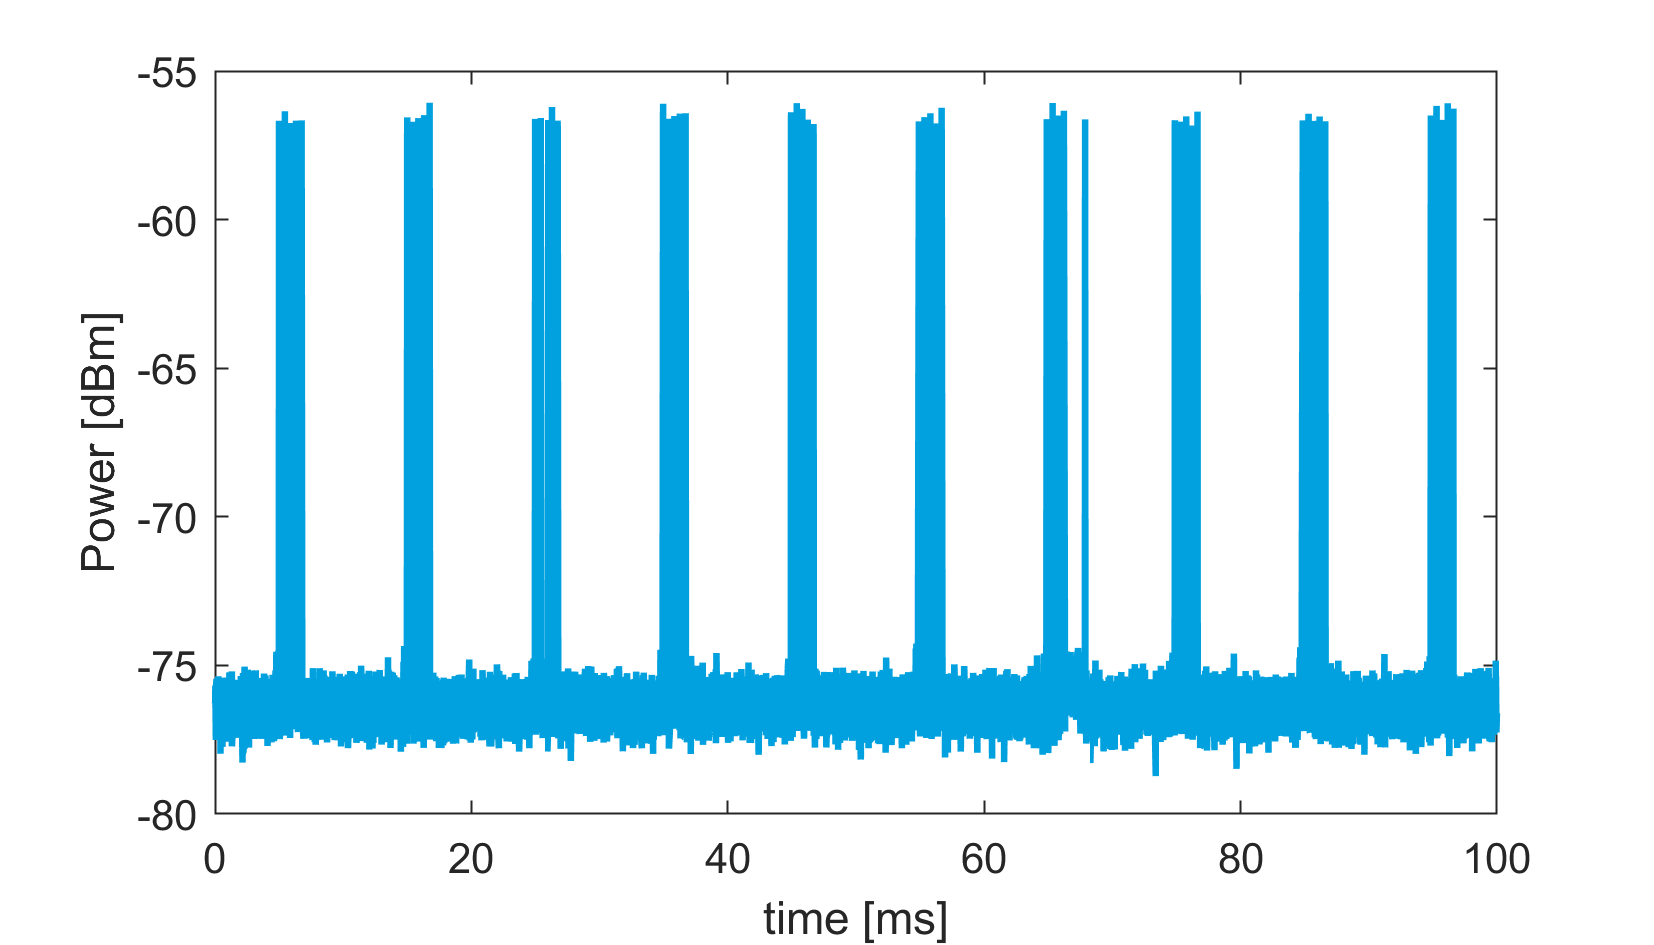
\includegraphics[width=0.49\textwidth]{trace_100.png}} \label{fig:m}
  \centering
  \subfigure[Zoomed trace of Figure (a)]{\includegraphics[width=0.49\textwidth]{{trace_100_zoom.png}}} \\
   \subfigure[Sweep time of 20ms]{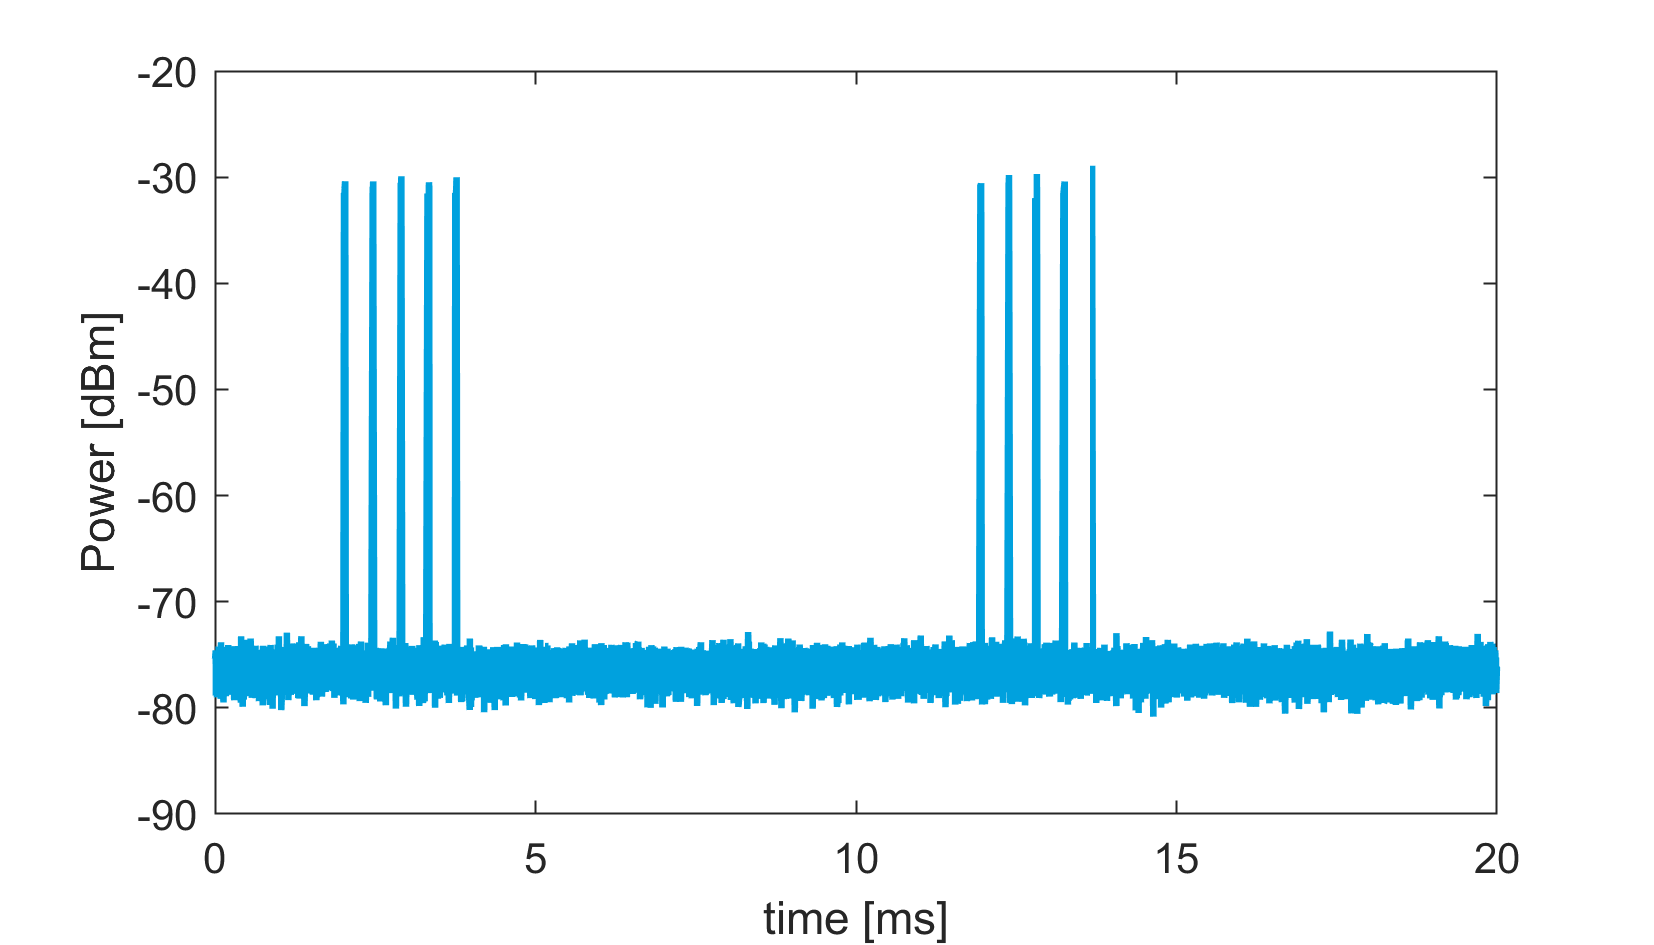
\includegraphics[width=0.49\textwidth]{trace_20.png}} \label{fig:n}
  \centering
  \subfigure[Zoomed trace of Figure (c)]{\includegraphics[width=0.49\textwidth]{{trace_20_zoom.png}}}
\caption{Trace}
\label{fig:rands}
\end{figure}




\subsection{Link Budget} \label{sec:lb}
The link-budget is necessary to design the complete end-to-end measurement system. Consider receiver blocking measurement and hence we require a blocking signal from the signal generator. Figure \ref{fig:link} explains the calculation of the levels within the system.

\begin{figure}[H]
\centering
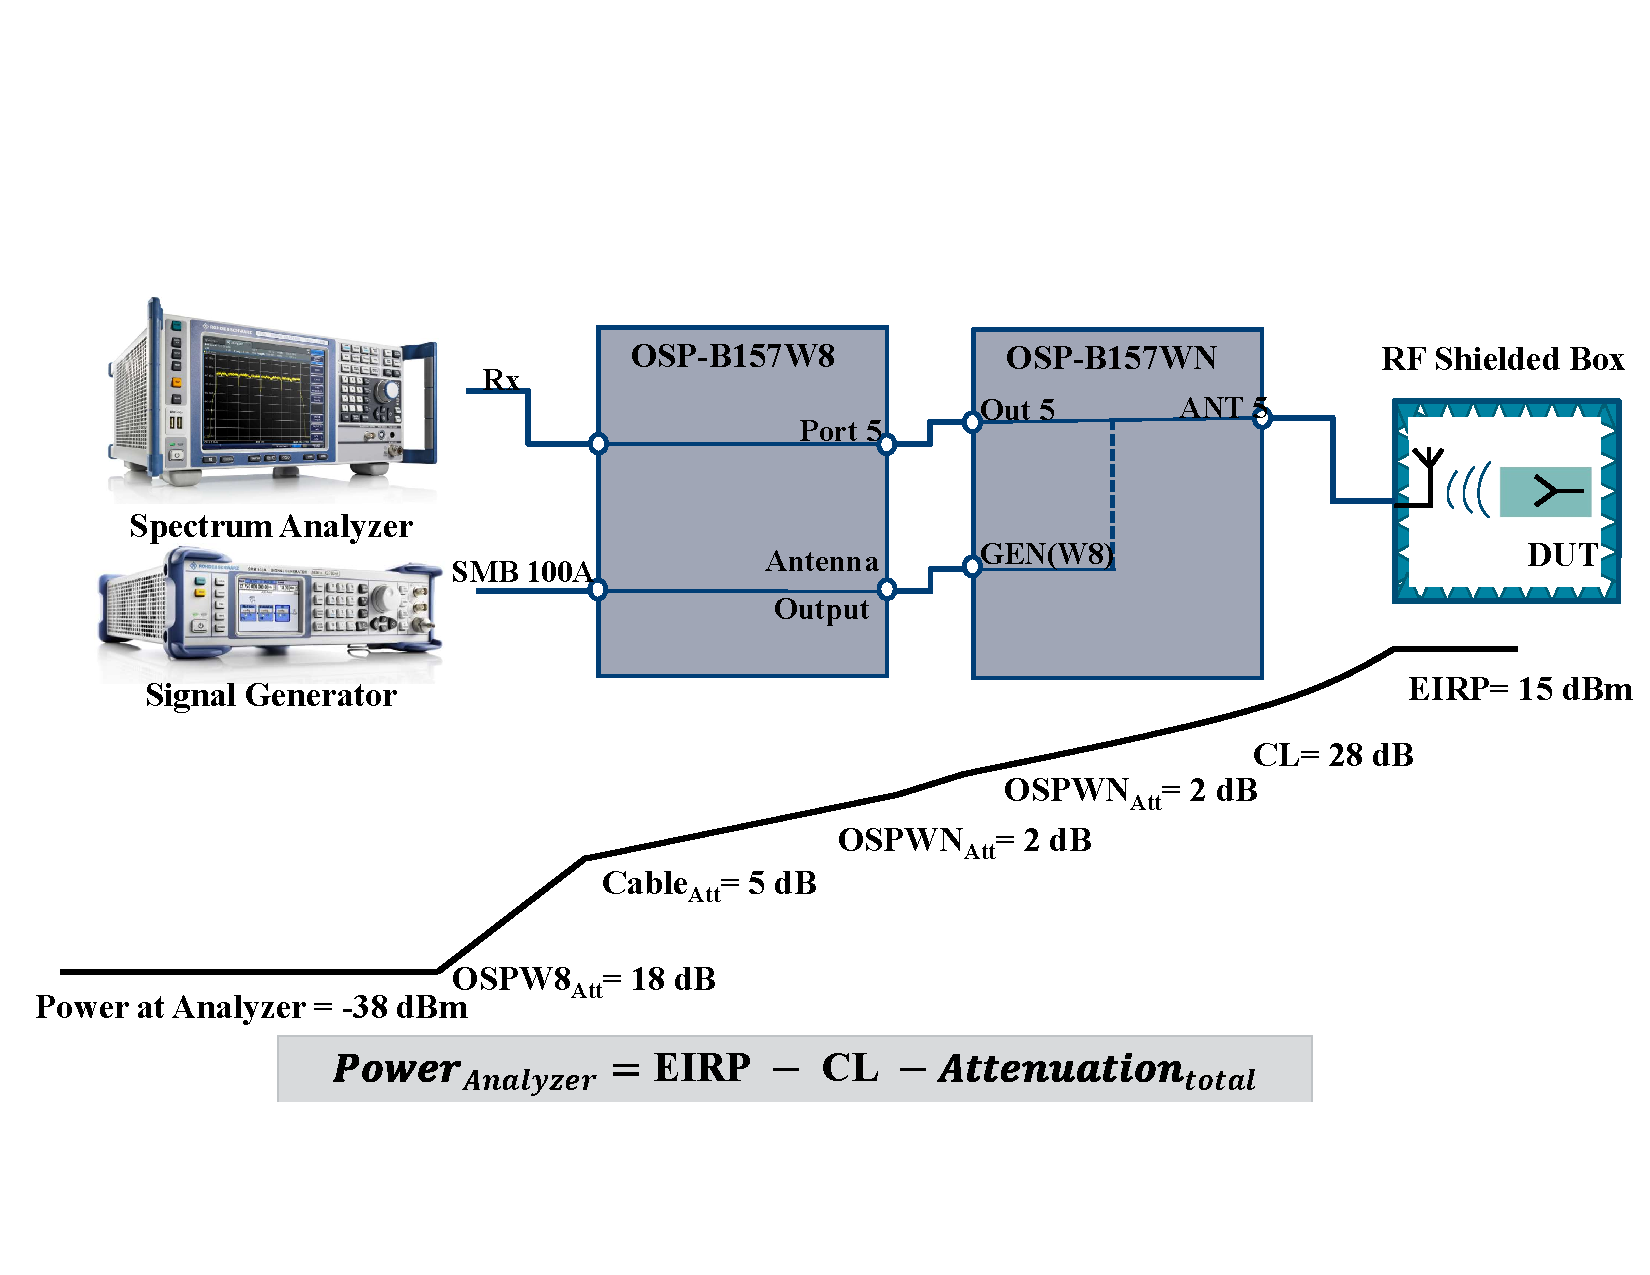
\includegraphics[scale = 0.6]{link_budget.pdf}
\caption{Link Budget diagram}
\label{fig:link} 
\end{figure}

Suppose the calculated power (i.e. a maximum of an average of \acs{RMS} burst power) at the analyzer is -38~dBm, total attenuation (switching modules and cables) is 25~dB and maximum \acs{EIRP} is 15~dBm. Then, by using the formula from the previous section \ref{eq:bl}, the coupling loss at ANT 5 is 28~dB. According to the standard, receiver blocking measurement requires a blocker level of -47~dBm in front of the \acs{DUT} port. Then, to find the value of the level at the generator, we need to calculate backward. Therefore the value at the generator would be given by equation \ref{eq:BL}.
\begin{equation}
\mbox{Blocker Level}_{\mbox{generator}}  = \mbox{Blocker Level}_{\mbox{DUT}} + \mbox{Attenuation}_{\mbox{total}} + \mbox{Coupling Loss} \label{eq:BL}
\end{equation}
Antenna Gain is already taken care of since the standard defined the power levels in front of the \acs{DUT} Antenna. Assume that the attenuation for this path is 18~dB. Therefore, by using the above formula, the power at the generator is 1~dBm. Attenuations are frequency-dependent and for the coupling loss, we can only rely on the used frequencies of the \acs{DUT}. Nevertheless, for the paths within the switching modules and the cables, the available calibration data for the specific frequency is used. As the blocker frequencies are not too far away (Figure \ref{fig:ax} ) from the in-band frequencies, the same coupling loss is considered.

\section{Optimization of Antenna Pair} \label{sec:opti}
Optimization of the probe antenna pairs is essential to ensure that the measurements are realized in optimal connections configurations with minimal losses and cabling again is not intended. The best selection of antenna pair is first implemented by performing a simulation on MATLAB\textregistered{} and later checking if the result coincides with the result from actual measurements. The later is also performed using the same algorithm. An important aspect to remember is that, as it is seen from the internal circuit diagram of OSPWN (\ref{fig:ospwn}) the antennas are arranged in pairs. And therefore, there are 15 possibilities for the optimum antenna pair selection.

\subsection{Simulation} 
To correctly perform the \acs{OTA} measurements in the \acs{RF} shielded box, a simulation for the link-budget analysis inside of the test chamber is required. This simulation, which is developed in MATLAB\textregistered{} environment will enable the choice of the best combinations of probe antenna pairs. For this purpose, a simulation of the transmission between the \acs{DUT} and all of the 6 probe antennas within the chamber, will allow a decision on the best associations between the instruments used for every test-case/measurement. The simulation also visualizes the effect of the positioning of a single-antenna \acs{DUT} within the chamber. The following parameters are considered in the simulation.
\begin{itemize}
  \item Configuration: The parameters of the chamber in the simulation e.g. the dimension of the chamber, antennas and, grid which holds the \acs{DUT}, placement of the antennas are tried to meet the existing system (Figure \ref{fig:room}). 
  \begin{figure}[H]
\centering
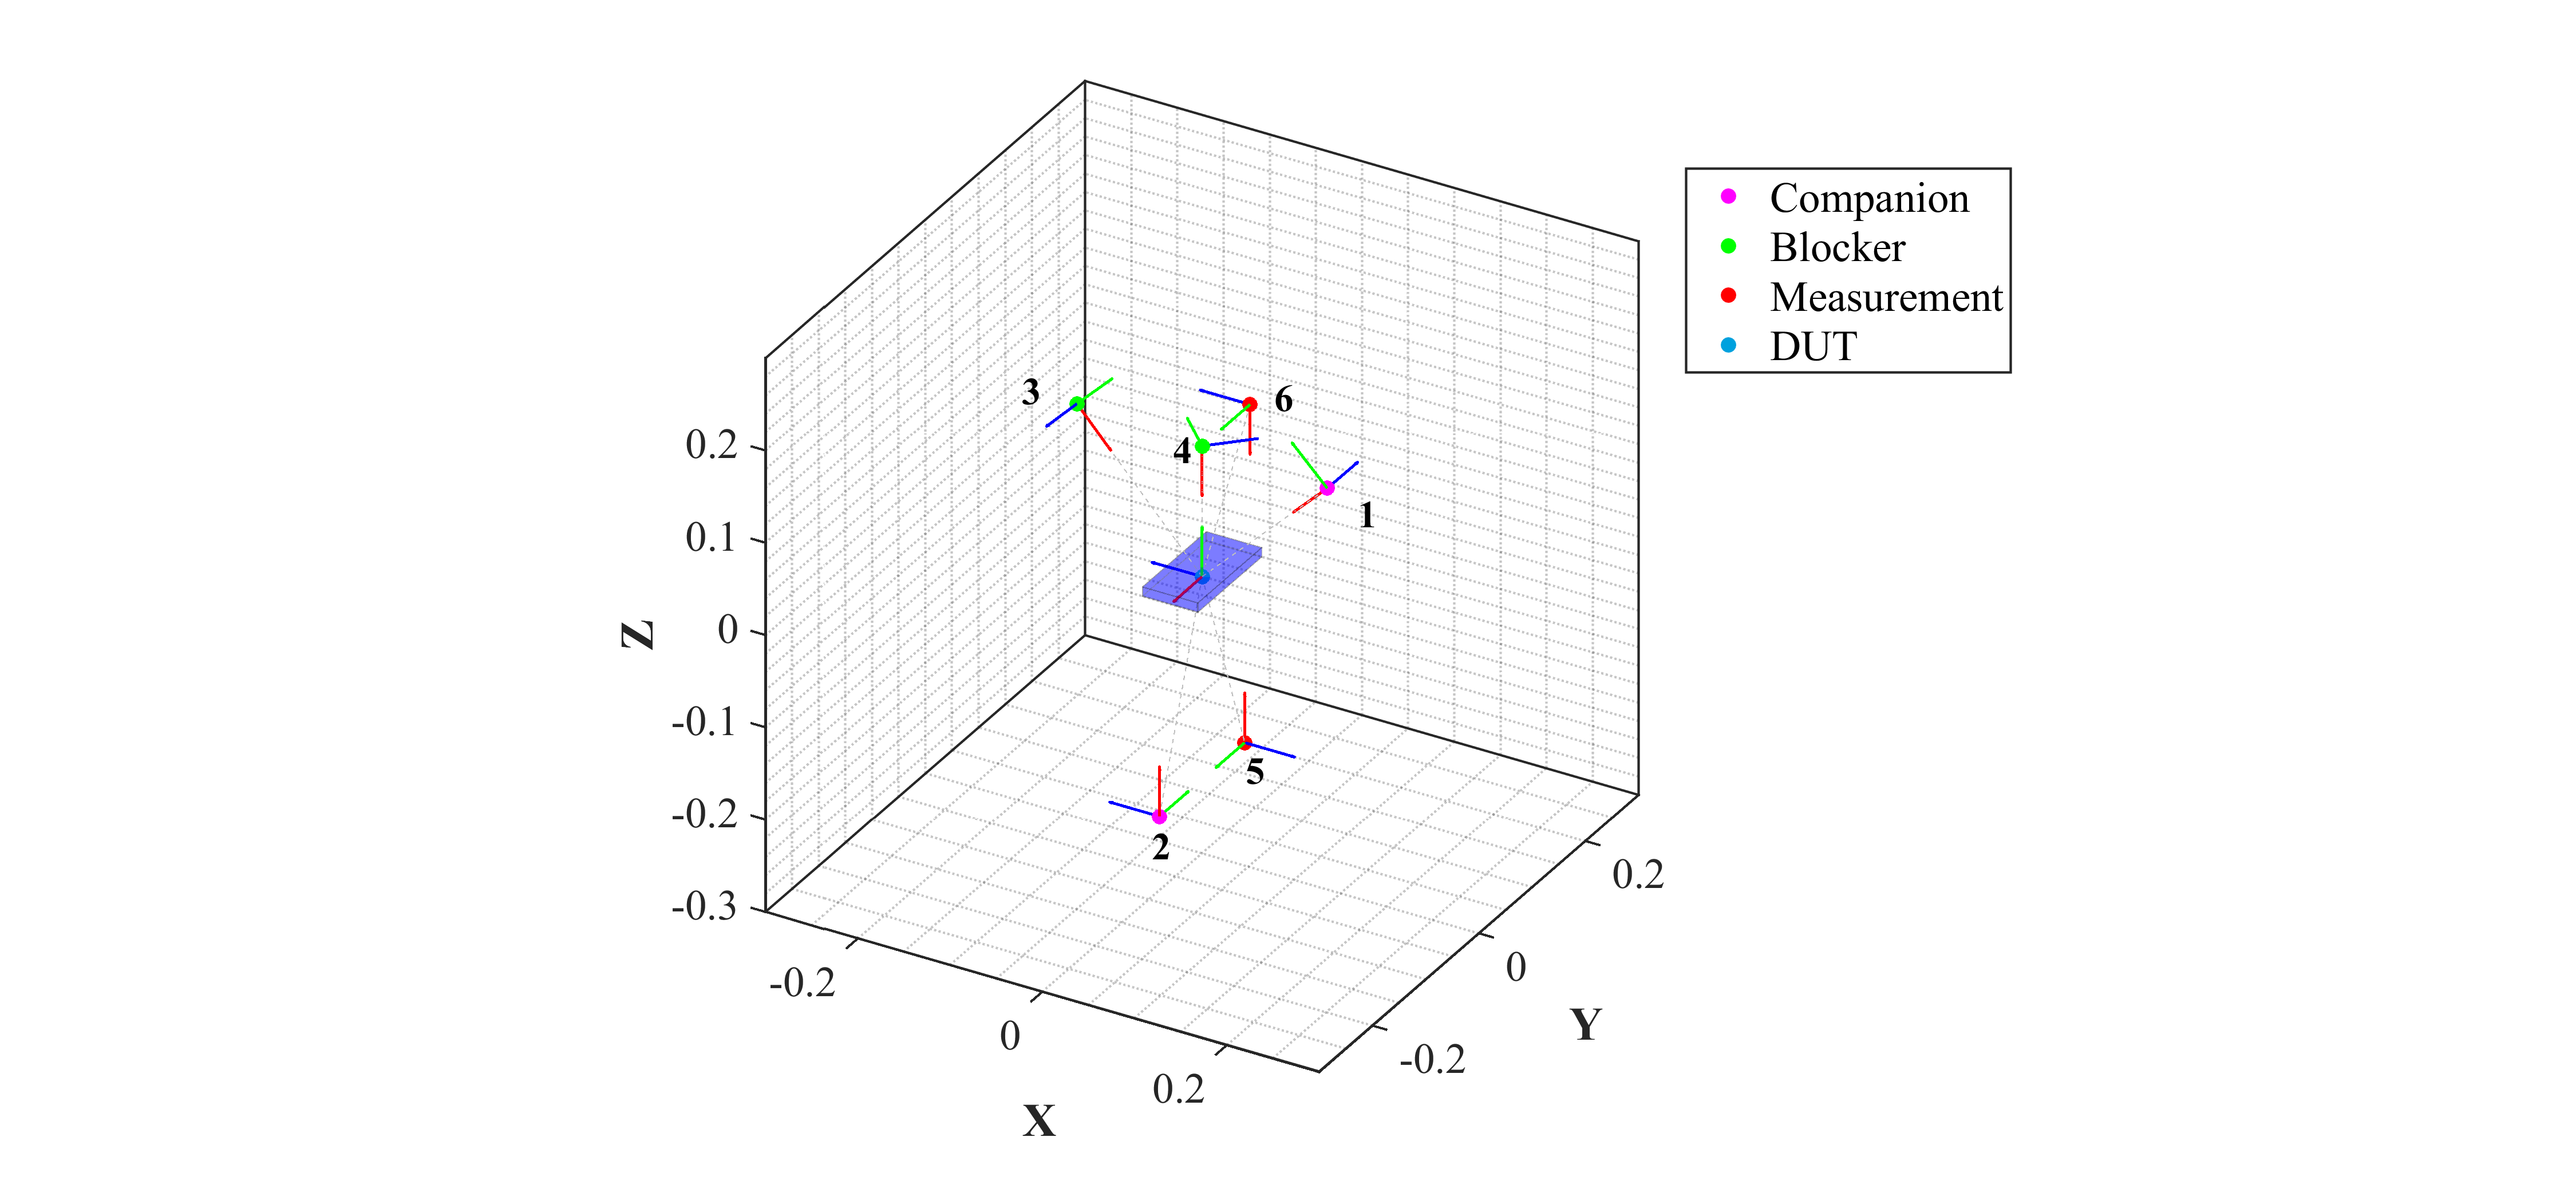
\includegraphics[scale = 0.53]{room.png}
\caption{Simulation diagram for the \acs{RF} shielded box}
\label{fig:room} 
\end{figure}

  \item \acf{FSPL}: This loss, which is given by the near field formula for path loss \cite{schantz}, is caused because of the distance separating the antennas and the frequency of the \acs{DUT} (2412 MHz). Theoretically, we are not supposed to perform measurements in \acf{NF} but since for we only have single-antenna pair in this case and we don't bother about the phase offset and phase curvature of the signal, the measurements are possible. Incase of multi-antenna \acsp{DUT} with antenna arrays, this is theoretically not possible due to the large antenna size resulting to perform measurements in the far-field. The test system is officially proposed for the use of single-antenna \acsp{DUT}. Nevertheless, we performed the tests with multi-antenna \acs{DUT} to examine if the theoretical effects play an important role.
 
  \item Antenna Polarization Loss: The polarization loss is due to the difference in positioning the antennas that directly influences the results of the choice of the best probe antenna pairs. We use the theory (section \ref{sec:pol}) and the MATLAB\textregistered{} functions to first compute the electromagnetic fields of each transmitter and receiver antenna in its local coordinates system based on their positions and types, then we find the horizontal and vertical components of the electric fields, which are needed for the MATLAB\textregistered{} function \textit{pollos} to compute the polarization loss between each two antennas (refer coordinates system \ref{pollos}).
  
  \item Antenna Gain (Transmitter gain ($\mbox{G}_{\mbox{TX}}$) and Receiver Gain ($\mbox{G}_{\mbox{RX}}$): For each used antenna, we compute and save its antenna pattern. Radiation patter for the vivaldi (probe) as well as dipole (\acs{DUT}) antenna is used from the MATLAB\textregistered{} antenna toolbox. Therefore the values are not exactly the same as the actual antennas used in the experimental setup. For the configuration for the room, we can locate a transmitter's coordinates in the local's coordinates system of the receiver and vice versa, so that from the look up table of the gain, we can use the local coordinates to find the gain of both the \acs{DUT} and the considered probe antenna. These values for the gain are added in the final formula  (\ref{eq:pl}) to compute the final loss between each probe antenna and the \acs{DUT}.
  
  \item Total Path Loss:
  The total path loss is given by the formula \ref{eq:pl},
  \begin{equation}  \label{eq:pl}
  \begin{split}
  \mbox{Path Loss (k,r)}  & = \mbox{FSPL} + \mbox{Polarization Loss} \\
  &= 10 \log\frac{4}{\frac{1}{(kr)^6}-\frac{1}{(kr)^4}+\frac{1}{(kr)^2}} - \mbox{G}_{\mbox{TX}} - \mbox{G}_{\mbox{RX}} + \mbox{Polarization Loss}
 \end{split}
 \end{equation}
   
   \end{itemize}
   
   
The simulation runs over 4000 random positions of the \acs{DUT} on the grid (\ref{fig:try}) inside of the chamber with randomly one of the three different orientation of its antenna as illustrated in the picture (link). For each position the total loss between the \acs{DUT} and each probe antenna is computed. Since for each instrument (Spectrum analyzer, companion or signal generator) a pair of probe antennas should be assigned for the connection, from which only one with the lowest path loss should be used for the measurement. Since we have 6 different probe antennas, and 3 instruments, there are 15 distinct different possibilities of combinations of 3 pairs of antennas, one pair for each instrument with one active probe antennas. From these 15 possibilities, the simulation allows a choice of the best combination with the lowest mean path loss, i.e. the mean of the minima of every 3 pairs out of the 15 is computed and then the best combination is found. Refer Figure \ref{fig:s} for the results from  15 antenna pair possibilities.

\begin{figure}[H]
\vspace{-3cm}
  \subfigure {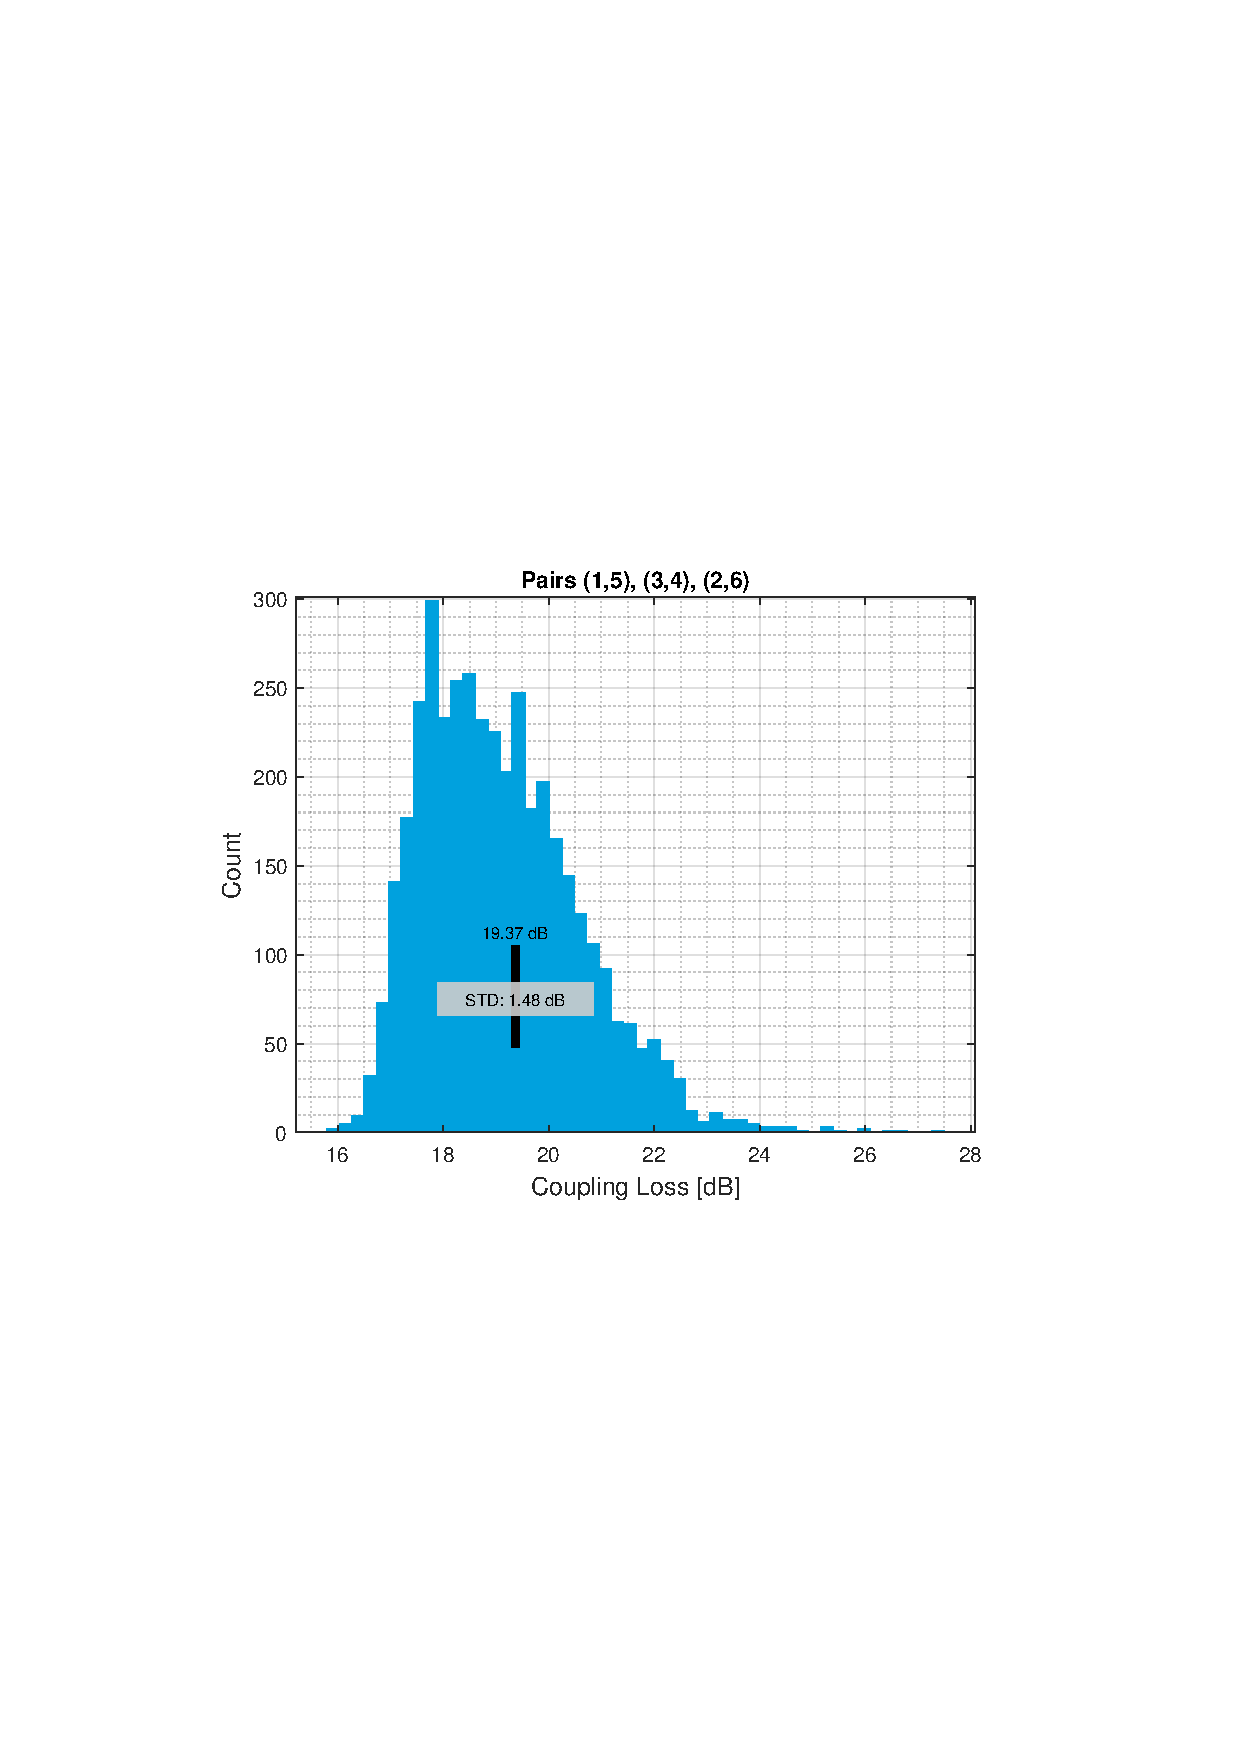
\includegraphics[width=0.65\textwidth]{simulation_best.pdf}} 
  \hspace{-3cm}
 % \centering
  \subfigure{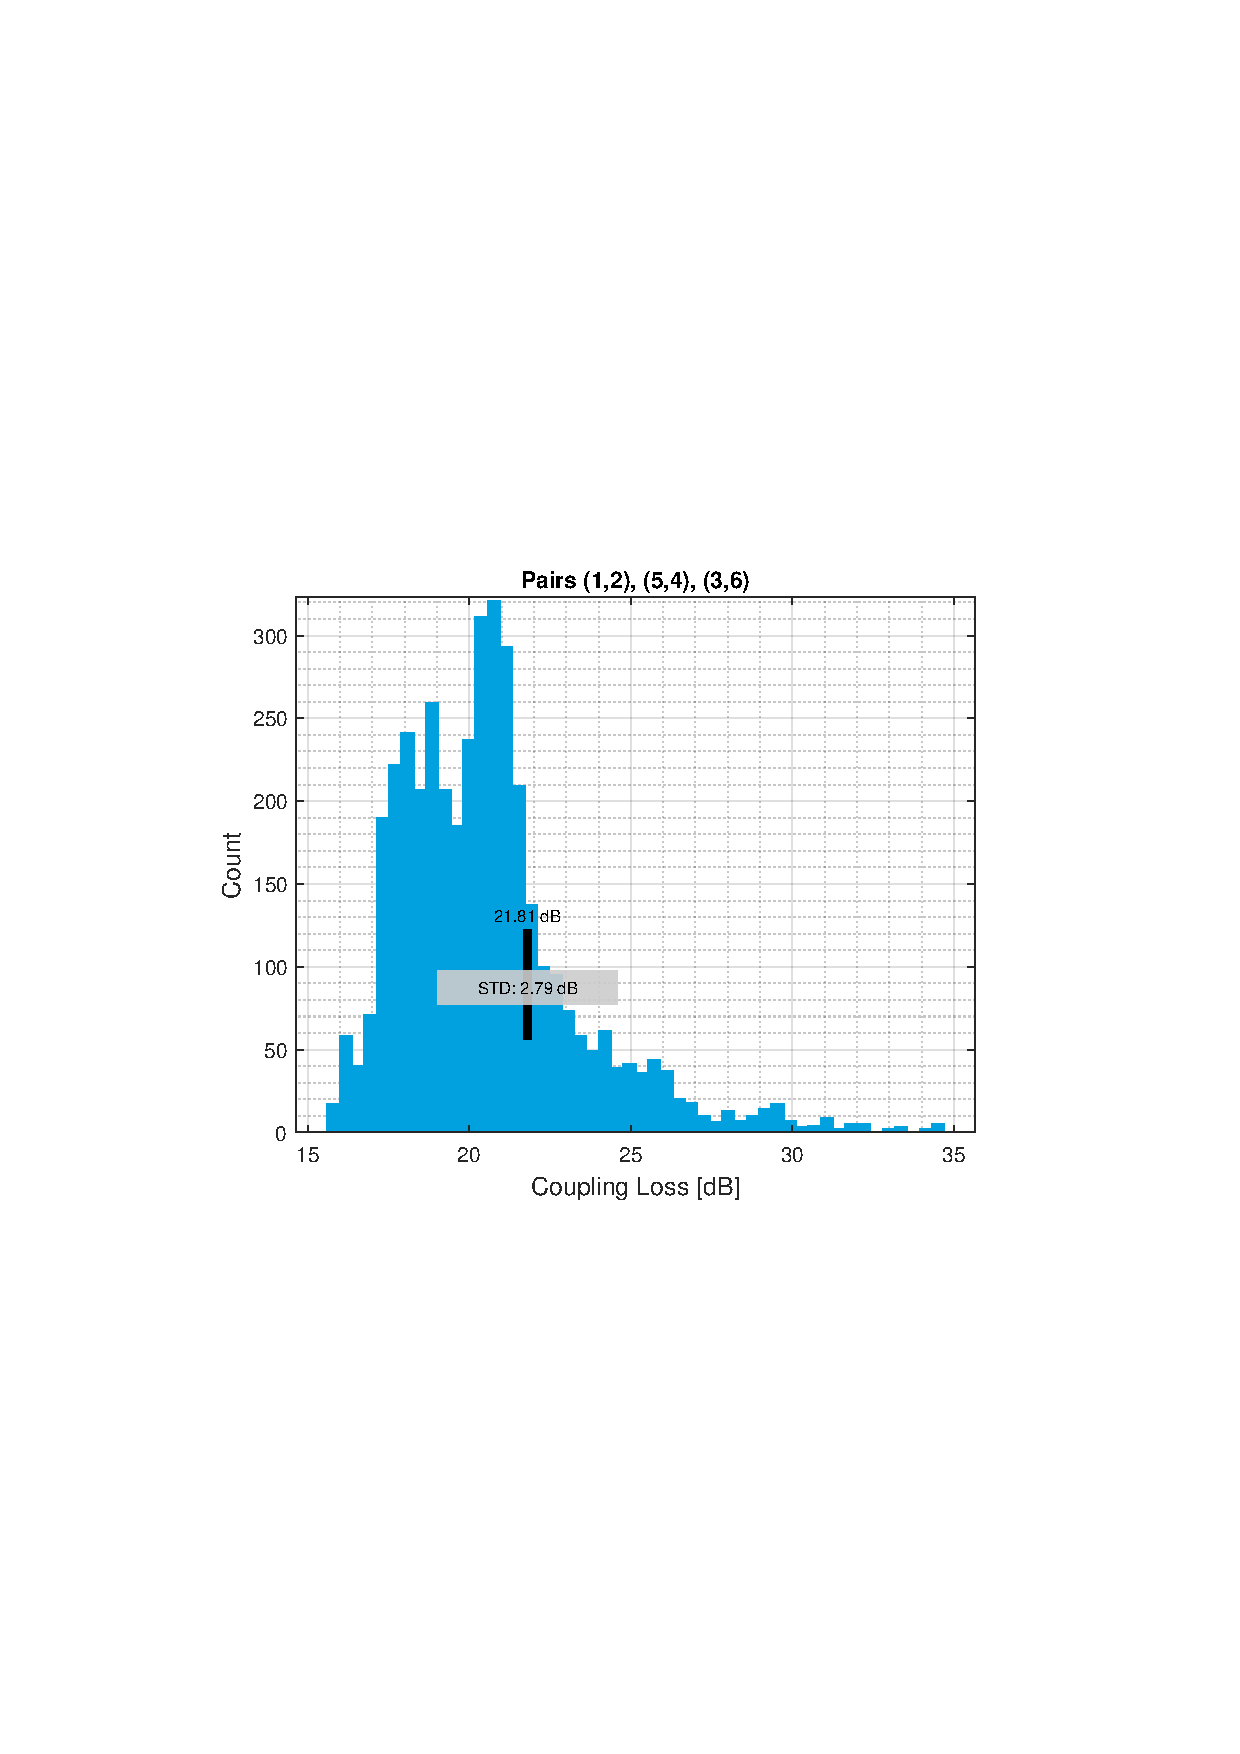
\includegraphics[width=0.65\textwidth]{simulation_worst.pdf}}
   \vspace{-3.9cm}
\caption{Figure in the left and right display the best and worst selection of probe antenna pairs after the simulation respectively}
\label{fig:simu}
\end{figure}



\subsection{Experimental Measurement} 
The small chamber in use is TS7124M which is a \acs{RF} shielding box with flat absorbers, which are used in order to minimize the effect of reflections. \acs{RF} shielded boxes are essential for reliably testing radio interfaces. The \acs{RS}\textregistered{} TS7124M \acs{RF} shielded boxes enable reliable and reproducible measurements when a shielded test environment is needed. \\

Normalization measurement is performed at 23 different positions (refer Figure \ref{fig:m}) inside the RF shielded box to find the range in which the coupling loss lies. The \acs{DUT} antenna is oriented in three different directions :horizontal, vertical and slant. Since the \acs{DUT} tray is small, it is enough to place the \acs{DUT} at 9 locations in horizontal and vertical orientation. And the remaining 5 locations are acquired when the \acs{DUT} antenna is in slant orientation. The limit of the coupling loss is defined by us and it states that the coupling loss must be less than 35~dB (refer \ref{eq:egBL}) so that an additional amplifier is not required in the hardware setup. For example, consider receiver blocking measurement. The equation \ref{eq:BL} explains the procedure to find the level of the blocking signal at the signal generator given the blocker level infront of the \acs{DUT}. Now, if the coupling loss is more than 35~dB (i.e 40~dB) then, the level at the blocker would be:
\begin{equation} 
\begin{split}
\mbox{Blocker Level}_{\mbox{generator}}  &= \mbox{Blocker Level}_{\mbox{DUT}} + \mbox{Attenuation}_{\mbox{total}} + \mbox{Coupling Loss} \label{eq:egBL} \\
& = -47 \mbox{~dBm} + 18 \mbox{~dB} + 40 \mbox{~dB} \\
& = 11 \mbox{~dBm} 
\end{split}
\end{equation}
Since we keep increasing the blocker level by steps of 1~dB from this value to check for 10\% \acs{PER}, the increase is usually around 15~dB from the value which is calculated (11~dBm). Thus, the limit of the level from the signal generator, which is +26~dBm will soon be reached. And therefore we would require additional amplifiers. In-order to not complicate the system by the use of additional amplifiers, the limit of 35~dB is set for the coupling loss. The figure \ref{fig:man} shows that Antenna 1 and 6, Antenna 2 and 3 and Antenna 4 and 5 result in minimum mean coupling loss as well as almost all bins as seen in the plot are below 35~dB of coupling loss. The remaining plots from the possible combinations are in Figure \ref{fig:n}.

\begin{figure}[H]
  \subfigure {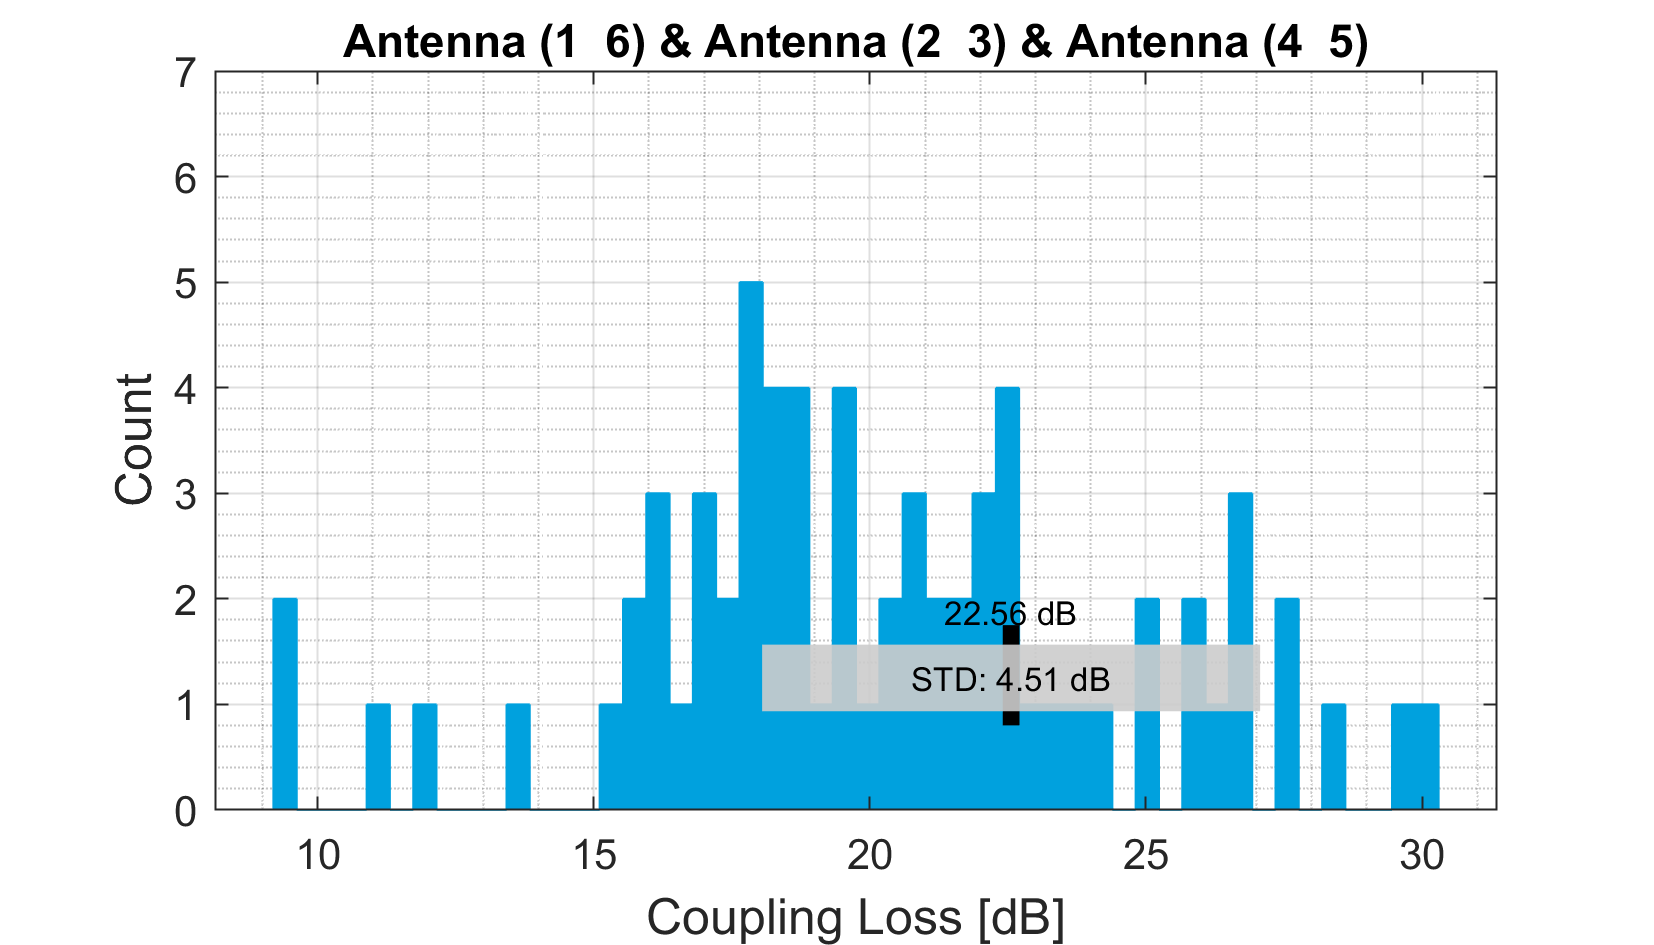
\includegraphics[width=0.5\textwidth]{manual_best.png}} 
  \subfigure{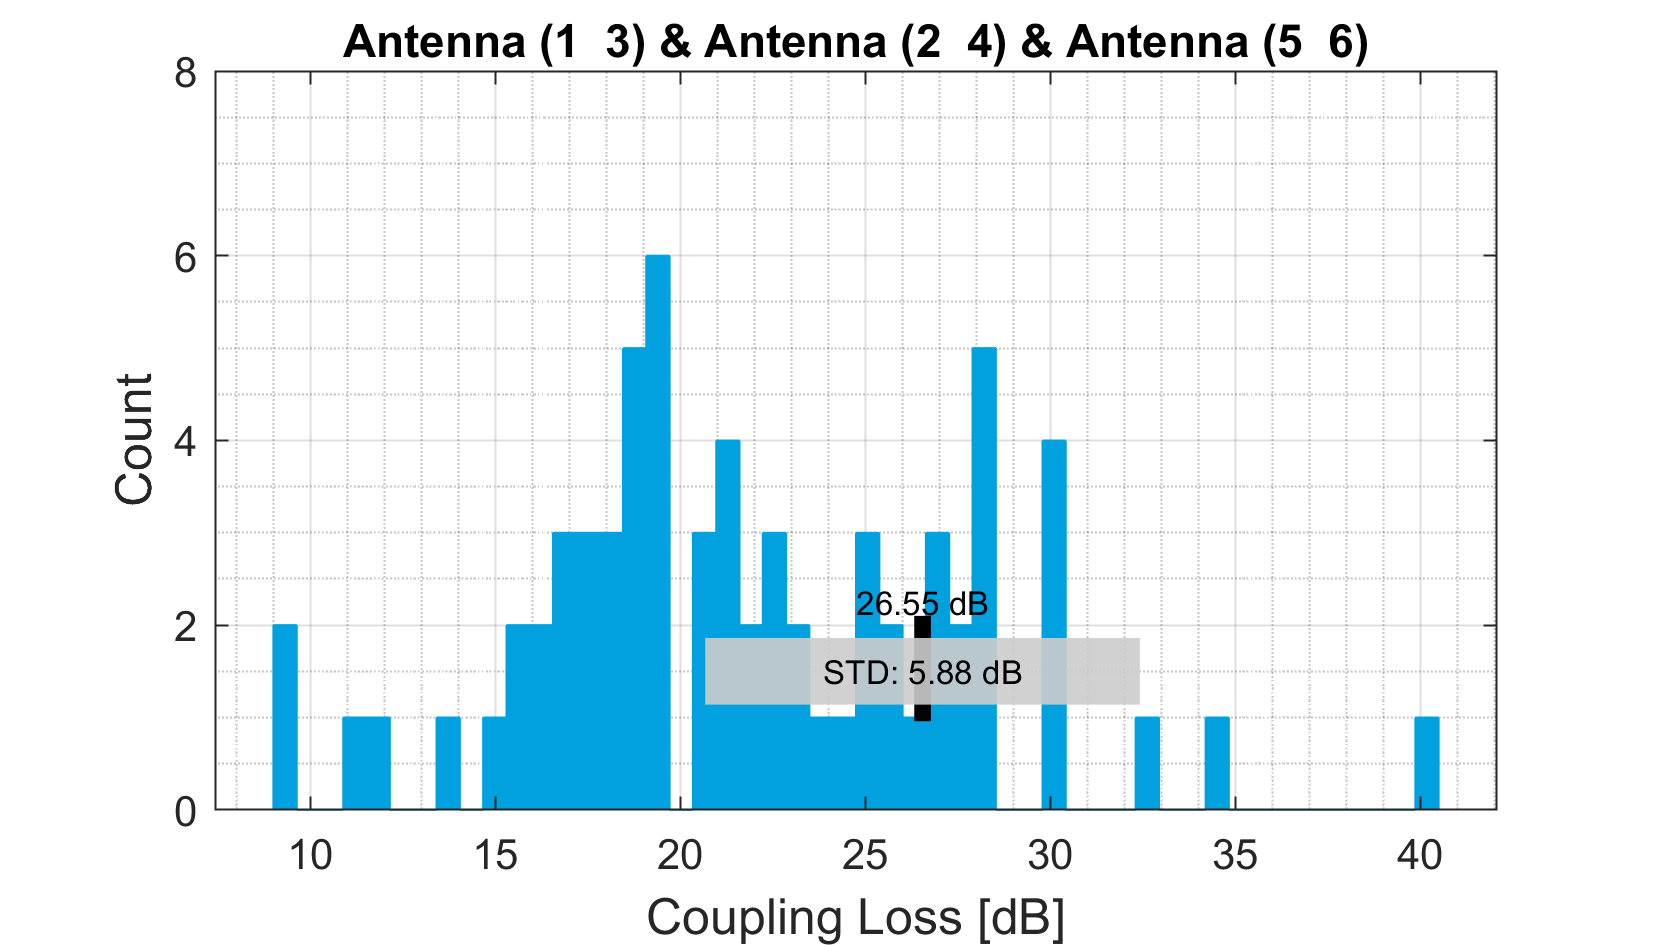
\includegraphics[width=0.5\textwidth]{manual_worst.png}}
\caption{Figure in the left and right display the best and worst selection of probe antenna pairs after the actual measurement respectively}
\label{fig:man}
\end{figure}

Comparing the simulation to the actual measurement, it can be noted that the range in which the coupling loss lies is approximately the same. Unfortunately the optimum pair does not match with pair resulting from the actual measurement. This can have several reasons: 
\begin{itemize}
\item Simulations take no charge of the reflections within the chamber. At some points in the chamber, there can be constructive or destructive interference. This increases the standard deviation because at some points we will see less power than simulations and at other we will see more power. These reflections can be due to the antenna mounting/holder and housing of the chamber. Because of the small size and flat absorbers of the \acs{RF} shielded box, the shielded box does not allow good anechoic performance.
\item The radiation pattern of the actual antennas might be different from the simulated antennas. This is because, simulation considered the radiation pattern from the MATLAB\textregistered{} antenna toolbox and not the actual used probe antennas which are manufactured at \acs{RS}\textregistered{}. In reality it can also happen that one probe antenna is 2~dB worse than the others. 
\end{itemize}



\section{Selection of Best Probe Antenna} \label{sec:sba}
The selection of the best probe antenna for each device depends on the coupling loss and the measurement test case. Isolation between the used probe antennas could be an additional parameter that may be important but this thesis does not consider it.  \\

Receiver blocking requires a signal generator and a companion device. The companion device is connected to COMP1 of the switching module OSPWN (refer Figure \ref{fig:ospwn}) and hence only antenna 1 and antenna 2 can be used for the companion device. The one with lower coupling loss would be considered as the best probe antenna. For the signal generator, only antenna 5 and 6 can be used since these paths go to GEN W(8) of the OSPWN. Again the one with less coupling loss will be the best probe antenna. Similarly, \acf{OBW} and \acf{PSD} measurements require a companion device and the spectrum analyzer. The best probe antenna is selected for the companion device from antenna 1 and antenna 2. The analyzer can then use any of the five remaining antennas.



















